\documentclass{article}

\usepackage{neurips_2019_author_response}

\usepackage[utf8]{inputenc} % allow utf-8 input
\usepackage[T1]{fontenc}    % use 8-bit T1 fonts
\usepackage{hyperref}       % hyperlinks
\usepackage{url}            % simple URL typesetting
\usepackage{booktabs}       % professional-quality tables
\usepackage{amsfonts}       % blackboard math symbols
\usepackage{nicefrac}       % compact symbols for 1/2, etc.
\usepackage{microtype}      % microtypography
\usepackage{graphicx}
\usepackage{lipsum}

\begin{document}
First of all, we would like to thank the reviewers for their critique concerning writing and novelty.  Regarding writing, we agree that sequencing and clarity can be improved.  We will restructure the paper and circulate it more broadly before resubmitting.  In addition, the reviewers have pointed out that novelty was either unclear or only clear upon reading the later sections.  This is, unfortunately, a fair criticism, and we will entirely re-write the introduction - in particular, to be clear about the paper's contribution.  Regarding novelty - in the realm of gaussian data, our paper "only" bridges two parallel and heretofore disconnected branches of research on latent space (from topic modeling and from Bayes nets), backporting the powerful PCA method to the Bayes net domain.  This in turn allows us to ask a "what if" with respect to generalization beyond gaussian variables, and potentially opens the door to non-linear feature detection (such as with autoencoders).  The outline of our contribution can be seen in figure \ref{fig:novelty} .  Let us consider novelty in detail.

Much of the prior work (e.g., Anandkumar et al., Wang and Blei) assumes that the observables are independent given the latent space. This is violated when they are driven by other observables, as in Figure \ref{fig:complicated}.  Nachman et al. couple the structure and latent space but use local cluster residuals.  In the current paper we combine these ideas, using the entirety of network residuals, while only assuming that the network nodes are independent given \textbf{\textit{both}} network structure and latent space.  Unlike Nachman et al., we also decouple structure learning form latent space learning.  This allows for further extensions: the latent structure can be learned using specialty feature-detection algorithms (e.g., autoencoders).  We also generalize learning to ordinal variables - an important advance from the point of view of real-world applicability.  Finally, we clarify the need of inferring the latent structure in order to improve the average causal effect estimates (ACE) - the causal field focused on ACE tends to assume "causal sufficiency" - that is, full observability of the data - but in practice this assumption is very strong and latent-space discovery methods are crucially important for ACE.

Regarding the empirical illustrations, we have other, more complicated models which were not included due to the lack of space. Figure \ref{fig:complicated} shows a case where the latent space is intertwined with the observables.  This could represent, for example, transcription factor proteins in a gene expression network.  Biological assays fail to cover many crucial data types at scale, and most experiments omit the majority of possible assays out of logistical and cost concerns.  The inter-dependence of latent and observable variables in Figure \ref{fig:complicated} means that certain approaches (e.g. Anandkumar et al., Wang and Blei) would not apply: the drivers of the outcome are not only dependent on the latent space but also on the drivers of latent space, confounding inference. For this model it is necessary to learn the connections of the drivers instead of assuming that only the latent variables drive them.

Regarding the comparison with other algorithms, we are not aware of any published implementation of methods that produce similar results to the algorithm that we are presenting (e.g. Nachman et al.).  This fact attests to the novelty by itself - we do provide an implementation on top of a popular Bayes net package.  We only have tangentially useful comparators.  We could compare the output of FCI (Glymour et al., 2019) to that of our algorithm.  FCI outputs mixed graphs (with directed and undirected edges) and can't be used to estimate causal effects directly, making for a qualitative comparison.  Focusing on ACE, we could compare treatment effect estimates obtained from ignoring the latent variables (e.g. using linear models) vs estimate from our algorithm after correcting for the latent confounders.

To conclude, we will work to revise the paper for clarity as described above.  Regarding novelty, we would like to ask the reviewers to consider our contribution in its totality and for its practical utility, rather than only by the scope of each individual advance taken in isolation.  The PB\&J sandwich is not diminshed by the use of known ingredients.  

\begin{figure}[ht!]
  \centering
    \begin{minipage}[t]{0.61\linewidth}
  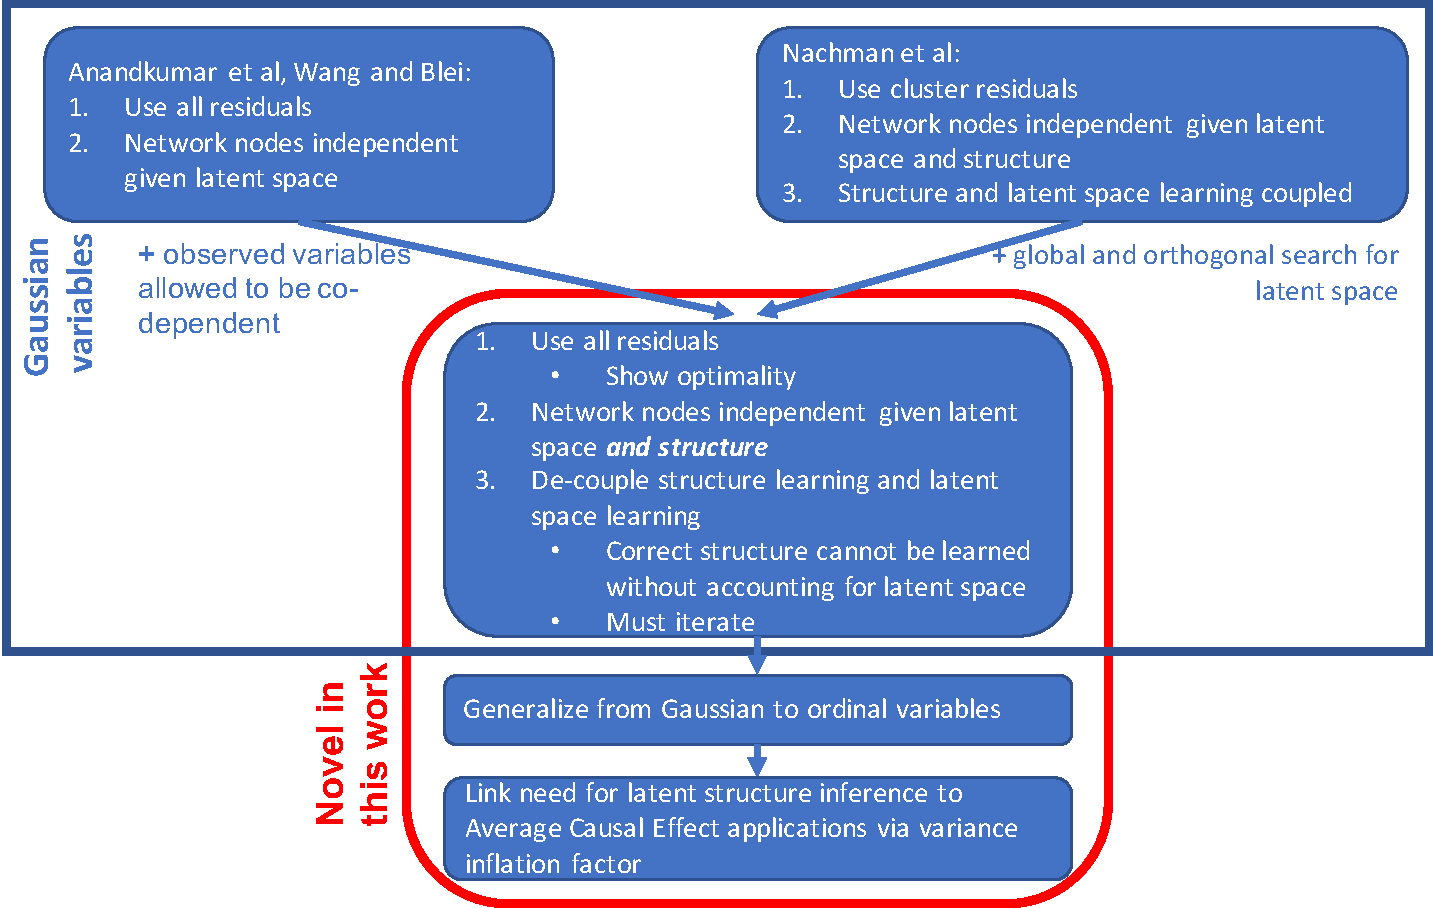
\includegraphics[scale=0.42]{./novelty.pdf}
    \caption{\label{fig:novelty}Overview of this work's contribution.}
  \end{minipage}
  \begin{minipage}[t]{0.38\linewidth}
  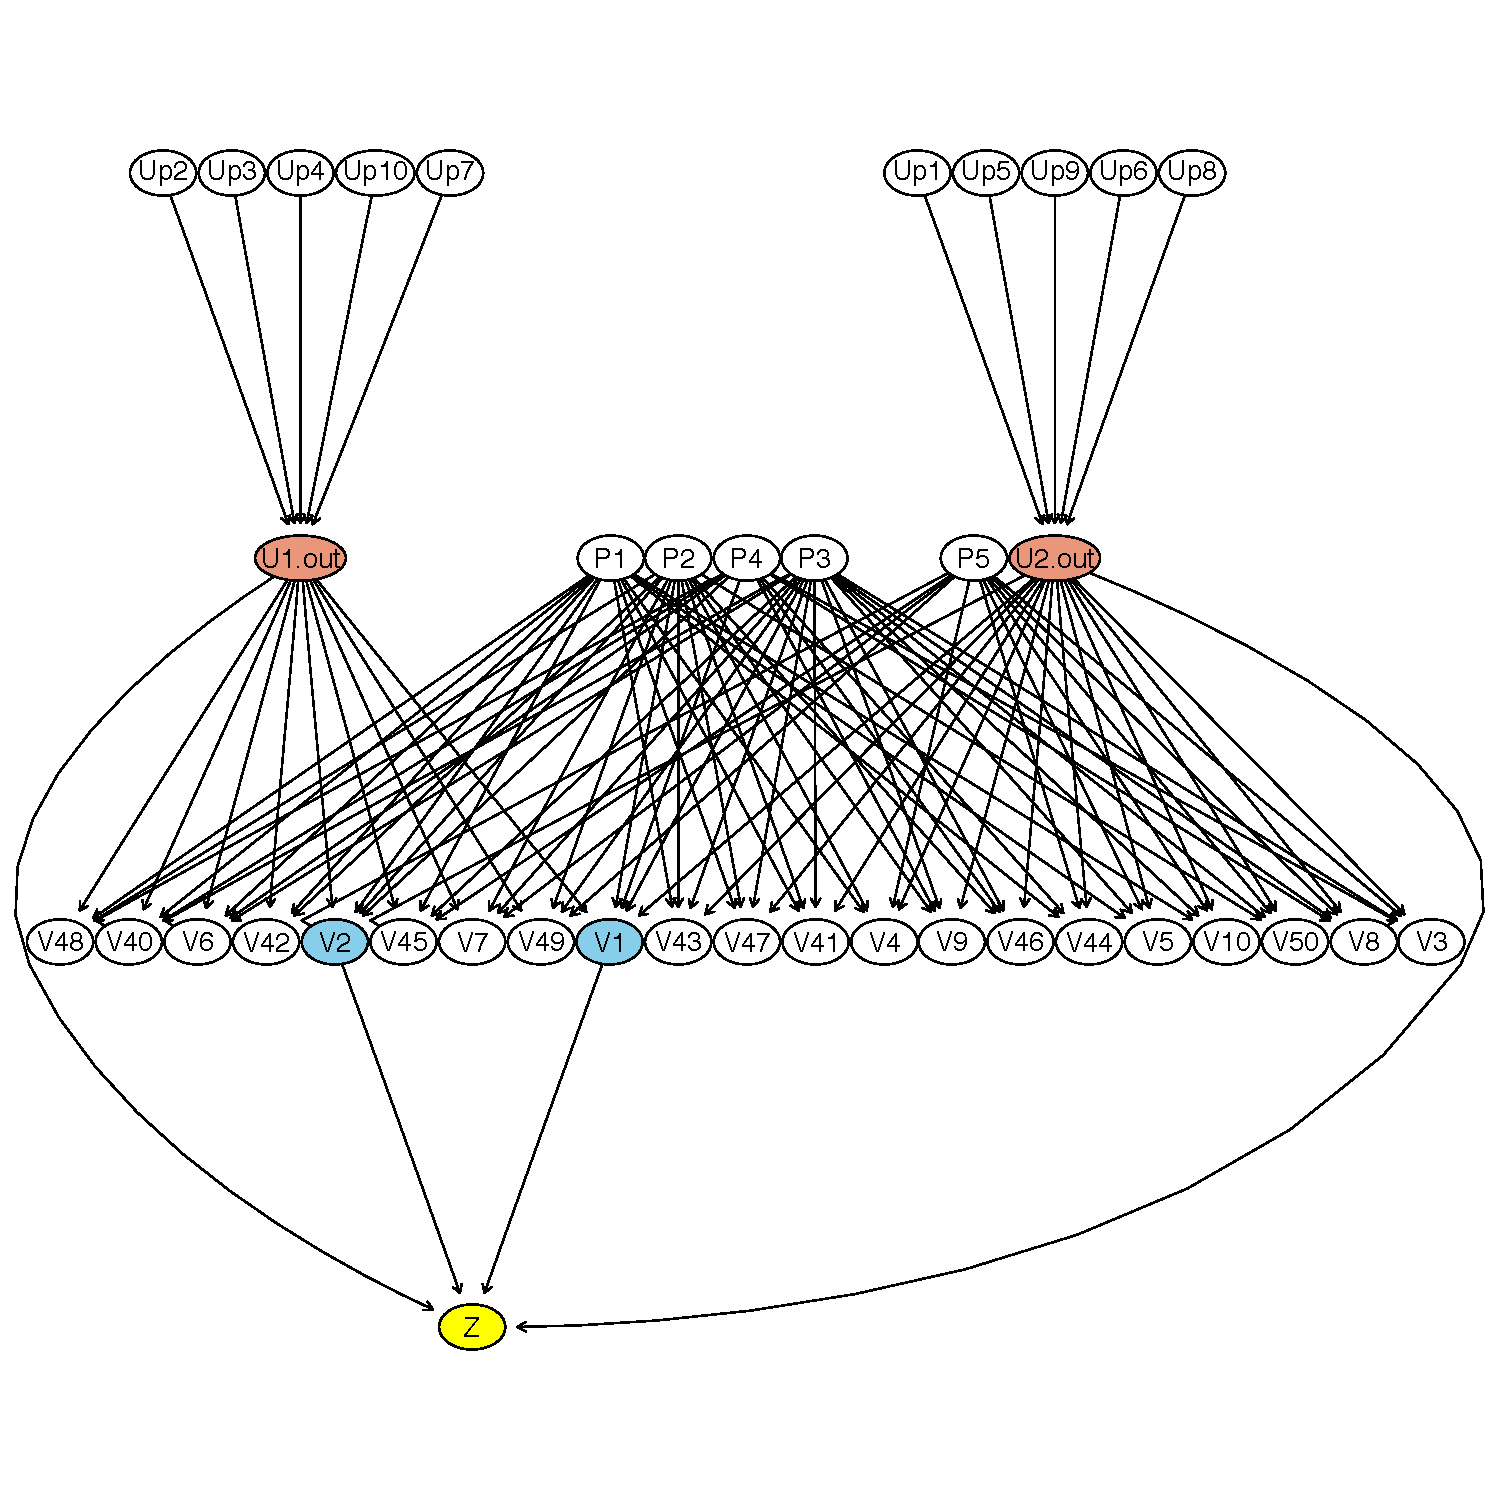
\includegraphics[scale=0.31]{./complicated_model.pdf}
    \caption{\label{fig:complicated}A more complicated model.}
  \end{minipage}
\end{figure}

\end{document}

